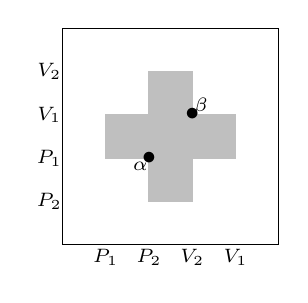
\begin{tikzpicture}[auto,scale = 0.55]
\draw (0,0) rectangle (5,5);
\draw [fill = gray!50,draw = gray!50] (1,2) rectangle (4,3);
\draw [fill = gray!50,draw = gray!50] (2,1) rectangle (3,4);
\node (P1a) at (1,-0.3) {\scriptsize{$P_1$}};
\node (P1b) at (2,-0.3) {\scriptsize{$P_2$}};
\node (P2b) at (-0.3,1) {\scriptsize{$P_2$}};
\node (P2a) at (-0.3,2) {\scriptsize{$P_1$}};
\node (V1b) at (3,-0.3) {\scriptsize{$V_2$}};
\node (V1a) at (4,-0.3) {\scriptsize{$V_1$}};
\node (V2a) at (-0.3,3) {\scriptsize{$V_1$}};
\node (V2b) at (-0.3,4) {\scriptsize{$V_2$}};
\node (dead) at (2,2) {$\bullet$};
\node (ina) at (3,3) {$\bullet$};
\node (al) at (1.8,1.8) {\scriptsize{$\alpha$}};
\node (be) at (3.2,3.2) {\scriptsize{$\beta$}};
\end{tikzpicture}
\quad\quad\qquad
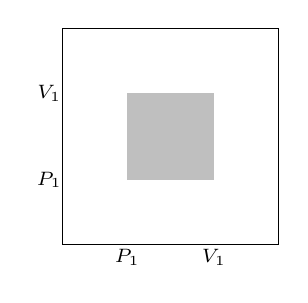
\begin{tikzpicture}[auto,scale = 0.55]
\draw (0,0) rectangle (5,5);
\draw [fill = gray!50,draw = gray!50] (1.5,1.5) rectangle (3.5,3.5);
\node (P1a) at (1.5,-0.3) {\scriptsize{$P_1$}};
\node (P2a) at (-0.3,1.5) {\scriptsize{$P_1$}};
\node (V1a) at (3.5,-0.3) {\scriptsize{$V_1$}};
\node (V2a) at (-0.3,3.5) {\scriptsize{$V_1$}};
\end{tikzpicture}